\documentclass{beamer} 
\usetheme{Warsaw}


\title{Inter-Packet Network Delays as a Time-Series Random Generator:}
\author{Micah Thornton, Neha Joshi, Qiliang Zeng}
\date{\today}


\begin{document}

\begin{frame}
\maketitle{}
\end{frame}

\section{Introduction}

\begin{frame}
\tableofcontents{}
\end{frame}
\begin{frame}
\tableofcontents[hideallsubsections, 	currentsection]
\end{frame}


\subsection{Random Numbers \& Applications}

\begin{frame}
\frametitle{History of Random}

\begin{figure}
\vspace{- 1 em}
{\tiny \textsc Figure 1: Ancient bone die used by Roman Empire circa 100-300 AD}

\begin{center}
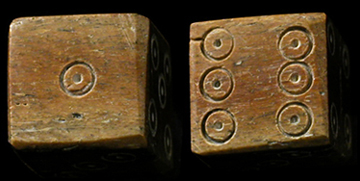
\includegraphics[scale=0.45]{images/ufdie.jpg}
\end{center}
\end{figure}

\vspace{- 1.5 em}
\begin{itemize}
		\item In ancient times, random values used for \textbf{gambling,  forecasting and fortune-telling}
		\item In modern times, they are used for \textbf{Security and Simulation}
		\item Process random iff all outcomes have equal probability of occurrence. 
\end{itemize}
\end{frame}

\begin{frame}


\begin{columns}

\begin{column}{0.5\textwidth}

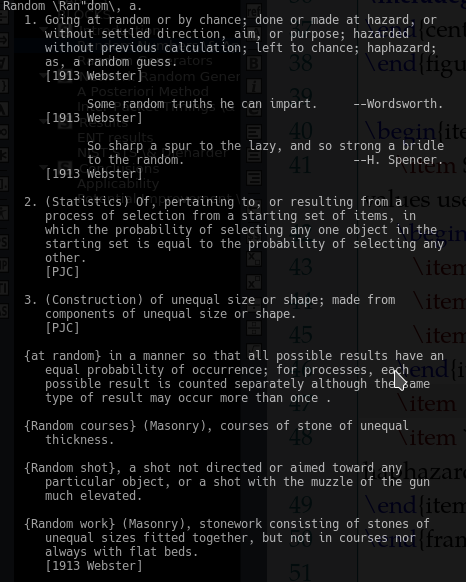
\includegraphics[scale = 0.5]{images/random-def.png}
\end{column}

\begin{column}{0.5\textwidth}
\end{column}

\end{columns}

\end{frame}


\

\subsection{Random Generators}
\begin{frame}
test
\end{frame}
\section{Network Random Generator}
\begin{frame}
\tableofcontents[hideallsubsections, 	currentsection]
\end{frame}
\begin{frame}
test
\end{frame}
\subsection{A Posteriori Method}
\begin{frame}
test
\end{frame}
\subsection{Inter-Packet Timings \& Data Production}
\begin{frame}
test
\end{frame}
\section{Results}
\begin{frame}
\tableofcontents[hideallsubsections, 	currentsection]
\end{frame}

\begin{frame}
test
\end{frame}
\subsection{ENT results}
\begin{frame}
test
\end{frame}
\subsection{NIST STS \& Dieharder}
\begin{frame}
test
\end{frame}
\section{Conclusions}
\begin{frame}
\tableofcontents[hideallsubsections, 	currentsection]
\end{frame}

\begin{frame}
test
\end{frame}
\subsection{Applicability}
\begin{frame}
test
\end{frame}
\subsection{Potential Improvement \& Future Work}
\begin{frame}
test
\end{frame}





\end{document}